\chapter{Used technology}

This chapter briefly describes the used technologies to implement a theft detection algorithm for vehicles. It introduces the Vehicle Connectivity Gateway and its web application Portal BetoTrack. After this the FMS standard is summarized.

\section{Vehicle Connectivity Gateway}
\label{sec::vcg}

The \textit{Vehicle Connectivity Gateway} (VCG) is a telematics and diagnostics unit. It connects a vehicle with different web portals and enables remote status monitoring of the vehicle as well as remote control actions. This unit can be build in cars, vehicles, trucks or agricultural machines \cite{VCG}.  

\begin{figure}[h]
    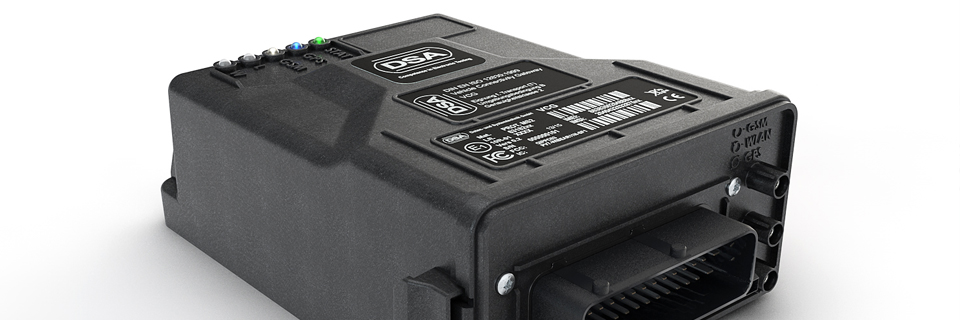
\includegraphics[width=1.0\textwidth]{src/pic/vcg_960x320px.jpg}
    \caption{VCG device \cite{DSA}}
\end{figure}

The VCG provides multiple communication mechanisms to transport data from the vehicle to the web:

\begin{itemize}
    \item GSM/UMTS Internet connection to the portal
    \item GPS/GLONASS satellite position detection
    \item WLAN for local diagnostics and additional functions
    \item One-Wire, RS232, digital and analog input for communication with sensors/transmitters
    \item CAN and Ethernet for ECU communication and diagnostics
\end{itemize}

Additionally the device has an build in accelerometer and build in battery to be independent of a vehicles power supply. We use the VCG to detect a theft of vehicles.

\section{Portal BetoTrack}

Portal BetoTrack is a tracking web application which allows to track vehicles equipped with VCGs. The app can be displayed in a browser an shows different states of a vehicle \cite{BetoTrack}. 
In context of this workshop the theft detection results should be displayed in this portal. The implementation of this was done by other groups of the workshop.

\begin{figure}[h]
    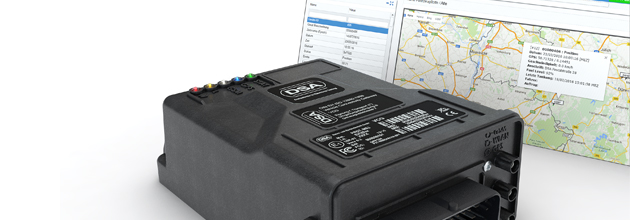
\includegraphics[width=1.0\textwidth]{src/pic/betotrack_630x220px.jpg}
    \caption{Portal BetoTrack \cite{BetoTrack}} 
\end{figure}

\section{Fleet Management System (FMS)}
\label{sec::FMSDef}

Fleet Management System (FMS) is a standardized interface for vehicle data. The FMS standard is supported by many big truck manufactures like Daimler, MAN Truck \& Bus, Scania, DAF Trucks, IVECO, Volvo Trucks and Renault Trucks \cite{FMS}.
The communication over the vehicle's CAN bus is standardized by the SAE J1939 network protocol.
FMS includes the following sensor values \cite{FMSStd}:

\begin{itemize}
    \item Vehicle improvement (all round)
    \item Vehicle speed (wheel based)
    \item Vehicle speed (from tachograph)
    \item Clutch switch (on/off)
    \item Brake switch (on/off)
    \item Cruise control (on/off)
    \item PTO (Status/Mode)
    \item Accelerator pedal position (0–100%)
    \item Total fuel used (litres since lifetime)
    \item Fuel level (0–100%)
    \item Engine speed
    \item Axle weight (kg)
    \item Total engine hours (h)
    \item FMS-Standard software version (supported modes)
    \item Vehicle identification number (ASCII)
    \item Tachograph information
    \item High-resolution vehicle distance
    \item Service distance
    \item Engine coolant temperature
\end{itemize}

Additional in version 2.0 the following values are also supported:
\begin{itemize}
    \item Environment temperature
    \item Driver ID
    \item Current fuel consumption
\end{itemize}

We use the FMS to have standardised values we can work with in our algorithm. In section \ref{sec::FMSUse} we describe which values we are using in our algorithm.


\clearpage